\documentclass[12pt,oneside,a4]{book}
\usepackage{hyperref}
\usepackage{float}
\usepackage{listings}
\usepackage{graphicx}
\usepackage{multirow}
\title{Mcabber User Guide}
\author{franky}
\begin{document}
\maketitle
\tableofcontents
\chapter*{Introduction}
This guide was written for users who are new to mcabber\cite{mcabber} which is a small
command line client for the Jabber protocol\cite{jabber} as an introduction. This introduction may
become a comprehensive guide to every aspect of mcabber later, but the first versions should only be
regarded as an overview of all features. Feel free to bug me with corrections of spelling errors or
with contributions to the content.
\paragraph{Conventions used in this guide:\\}
\begin{tabular}{ c p{10cm} }
	\verb+/command+ & This is a command for mcabber which can only be executed during runtime.\\
	\verb+command+ & A command for mcabber which can be given in the configuration file, too.\\
	\verb+$command+ & The \$-sign precedes shell commands.\\
	\textit{variable} & This is a variable which can be set in the configuration file or during runtime. \\
\end{tabular}
\chapter{Basic Usage}
After installing mcabber, you should create a configuration file first. The easiest way of doing this
is to copy the sample configuration file\cite{samplerc} to \~{}/.mcabber/mcabberrc. Then, you only have to change the variables
\textit{username} and \textit{server} before you can, finally, start mcabber. When the Login was successful,
mcabber might look similar to the following screenshot:\\
\begin{figure}[h!]
	\centering
	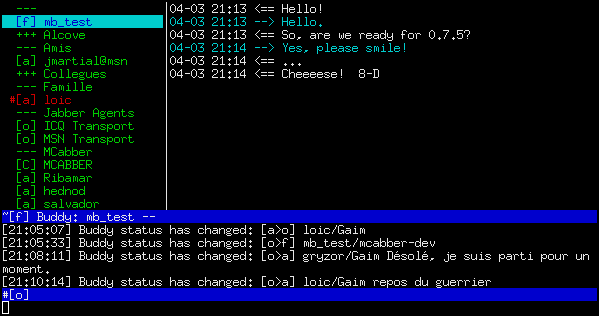
\includegraphics[scale=0.8]{guide}
	\caption{screenshot of mcabber}
	\label{fig:screenshot}
\end{figure}
The screen is divided into 4 regions: The roster(sometimes called buddy list) in the upper left,
the chat window/buffer in the upper right, the input line at the bottom and the log window above the
input line. Those two blue lines which are below and above the log window are status lines. The lower one
displays the general mcabber status and the upper line the status of the selected contact.
The screenshot shows mcabber in "chat mode" which can be entered by pressing enter or sending a message
when a contact is selected. Leaving chatmode is done by pressing Esc. To move between your contacts, you
can use the buttons Pg Up/Pg Down. If you look at the roster of the screenshot, you will notice that the
contact "loic" is marked red. That's the default for the "unread" color, so "loic" sent a message to
you, but you have not read it, yet. Moving by pressing Pg Down would need 6 key presses, so it might be faster to use
\verb+/roster unread_next+ to quickly jump to the next unread buffer. Which brings us to the interface of mcabber.
Since mcabber has only one input line, there has to be some way of distinguishing mcabber commands from normal text
messages. As you might have guessed already, all mcabber commands start with a slash, while any other line which you
have entered will be sent as a message to the selected buddy. You won't find a complete list of all commands here,
since mcabber has already got a great help system. It's at your fingertips when you enter \verb+/help+.
Furthermore, you can choose the language of the help system by setting \textit{lang} to de, en, fr, it, nl, pl, ru or uk.
\section{Multi-user Chat}
Jabber offers more than other one-on-one chats. There is an extension\cite{xep45} which adds many-to-many chat,
very similar to systems like IRC. Mcabber can participate through the command \verb+/room+. If you happen to
find big rooms, you should play a bit with \verb+/color muc+  to make the conversation more readable.
Last but not least, you might be interested in the channel mcabber@conf.lilotux.net as a new mcabber user.
Feel free to drop by and tell us about your experiences with mcabber or this guide!
\section{Transports}
Transports, also known as Gateways, are Jabber server components which are used for translating your Jabber messages
for proprietary networks like ICQ, AIM or MSN. At the time of writing, mcabber can't register transports, but,
if you've registered a transport with another client, you'll be able to use them within mcabber.
Transports are, basically, just another contact on your roster. Thus, using transports is done by sending your status,
maybe explicitly with \verb+/status_to+.
\section{Symbols}
Most users may be puzzled when they see all those different characters in the roster, the status bar and
in the chat window for the first time. Some of those symbols might be obvious, but others aren't descriptive at all.
So, here is a list of all characters and their meanings, structured per window where they were taken from. \\
\begin{tabular}{c  c}
	\begin{tabular}{|c | l|}
		\hline
		\multicolumn{2}{|c|}{Roster}\\
		\hline
		Symbols & Rosteritem \\ \hline
		\verb+---+	& unfolded Group \\
		\verb-+++- & folded Group \\ \hline
		\verb+[ ]+ & buddy or chat room(MUC) \\
		\verb+{ }+ & buddy who can't see your status \\
		\verb- + - & buddy is typing \\
		\verb+ . + & buddy stopped typing \\
		\verb+ _ +  & buddy status: offline \\
		\verb+ o + & buddy status: online \\
		\verb+ a + & buddy status: away \\
		\verb+ d + & buddy status: do not disturb \\
		\verb+ n + & buddy status: not available\\
		\verb+ f + & buddy status: free for chat \\
		\verb+ ? + & buddy status unknown \\
		\verb+ x + & muc status: not connected \\
		\verb+ C +  & muc status: connected \\
		\hline
	\end{tabular}
	&
	\begin{tabular}{|c | l|}
		\hline
		\multicolumn{2}{|c|}{Chat Window} \\ \hline
		Symbols & Meaning \\ \hline
		\verb+-->+ & sent message \\
		\verb+<==+ & received message \\
		\verb+~+	& message was encrypted with GPG\\
		\verb+O+	& message was encrypted with OTR\\
		\verb+***+ & info message \\
		\verb+#<#+ & error message \\
		\hline
	%\end{tabular}
	%\begin{tabular}{|c | l|}
	%	\hline
		\multicolumn{2}{|c|}{Upper Status Line} \\ \hline
		Symbols & Meaning \\ \hline
		\verb+~+ & chat mode enabled \\
		\verb+*+ & buffer is scroll-locked \\
		\verb+[C]+ & chatstate: composing \\
		\verb+[A]+ & chatstate: active \\
		\verb+[I]+ & chatstate: inactive \\
		\verb+[P]+ & chatstate: paused \\
		\verb+[G]+ & chatstate: gone \\
		\hline
	\end{tabular}
\end{tabular}
\chapter{Logging}
Some people write their diaries to remember special moments. Others merely save their chat logs,
which are often full of personal details, too. Of course, mcabber can keep your chat history
and fortunately, the format of these logs is easy enough to read with your
favourite text editor. Moreover, searching is possible with standard unix tools like \verb+$grep+.
\section{Enable Logging}
To enable logging, you'll have to add some lines to your configuration file:
\begin{lstlisting}
set logging = 1
set load_logs = 1
\end{lstlisting}
Those variables tell mcabber to log the chat history and to load old logs when you restart it.
Please note that there are a lot of other variables affecting logging. You can e.g. choose whether
you want to log Multi-user Chats(\textit{log\_muc\_conf}) or whether you want to log status changes(\textit{logging\_ignore\_status}).
You'll find them all in the sample configuration file\cite{samplerc} if you search for "History Logging".
\section{Grouping logs}
If you know other instant messengers, you might be used to a concept called "metacontacts".
They can be used to group users, which have multiple representations in your
roster (e.g. because they have work and home accounts). Unfortunately, mcabber doesn't support
metacontacts yet, but at least you can group the history of different contacts together.
This basically works by merging those histories and then creating a symlink frome one to the other.
Here's an example with the histories of foo\_work@jabber.org ond foo\_home@jabber.org:
\begin{lstlisting}
$ cd ~/.mcabber/histo/
$ merge_history.py foo_work@jabber.org foo_home@jabber.org > foo
$ mv foo foo_home@jabber.org
$ rm foo_work@jabber.org
$ ln -sf foo_home@jabber.org foo_work@jabber.org
\end{lstlisting}
The script merge\_history.py is included in the mcabber tarball.
\section{Converting centerim logs}
You've got old centericq\cite{centericq} or centerim\cite{centerim} logs and want to keep
them in mcabber? There's a script called cicq2mcabber.pl in the contrib directory of the mcabber
tarball which can be used to do that. Now you only have to figure out where exactly
centerim saves the history of a particular contact(somewhere under \~{}/.centerim/),
convert this file to the mcabber history format and save it to \~{}/.mcabber/histo/ with the
Jabber ID as the filename.
\chapter{Scripting}
This chapter will introduce you to the scripting facilities of mcabber.
\section{Aliases}
Aliases are used to map complex commands to a word. \verb+/roster search+ is one of the commands worth remapping
because it will be used every day. If you want to remap it to \verb+/rs+,
issue the command \verb+alias rs = roster search+.
\section{Internal Hooks}
Internal Hooks can be used to let mcabber execute commands when a special event occurs.
At the time of this writing, only 2 hooks were defined:
\begin{itemize}
	\item \textit{hook-post-connect}
	\item \textit{hook-pre-disconnect}
\end{itemize}
The time of the execution is self-explaining, just set those variables to the command you want
to execute.
\section{External scripts}
Mcabber will execute the external script specified in the variable \textit{events\_command} whenever a new
message is received. It will be called at least with 3 parameters:
\begin{enumerate}
	\item MSG or STATUS
	\item	IN, OUT or MUC if the first argument was MSG or one character of "\_OFDNAI" if the first argument was STATUS
	\item The JID which triggered the event
	\item (optional) filename of the file which contains the message body
\end{enumerate}
If you need the message body for your event script, you'll have to set the option \textit{event\_log\_files} to 1.
The script has to delete that file after it processed it. To execute mcabber commands,
you'll have to compile mcabber with FIFO support(\verb+$./configure --enable-fifo+). Then activate it by setting the
variable \textit{fifo\_name} to the filename of the fifo in your config file. There will be some verbose debug
output in the logging window if you don't set the variable \textit{fifo\_hide\_output} to 1.\\
There is another variable which might be interesting for the developer of external scripts.
If \textit{statefile} is set to a filename, mcabber saves the JIDs of all unread buffers to that file, one per line.
\chapter{Encryption}
Encryption is one of the greatest advantages of Jabber compared to similar
"legacy" networks like ICQ, MSN, AIM, etc. With encryption, you'll be able
to communicate in hostile network environments with a clear conscience,
because almost nobody will be able to spy on you. Practically, every connection
which is established when using the Jabber protocol could be encrypted.
First of all, you can connect to your Jabber server via ssl, which will
prevent anyone between you and the server from sniffing your plaintext
messages or your password. In mcabber you could enable this feature by adding
\begin{lstlisting}
set ssl = 1
set ssl_verify = -1
\end{lstlisting}
to your configuration file.
The next step is server to server encryption, which you can't control,
unless you're the admin of your server. So, theoretically it would be possible
to spy between Jabber servers, or maybe your buddy doesn't use an ssl
connection. Of course, if you are truly paranoid, you won't trust the
server admins but only your buddy. So, to encrypt messages between you and your
buddy, end-to-end encryption can be used. There are two protocols for
accomplishing this: The first one is OpenPGP/GnuPG, which is a semi standard\cite{xep27}
in the Jabber world. The other protocol is Off-the-Record(OTR) Messaging, which was
designed by cryptographers Ian Goldberg and Nikita Borisov\cite{otr}. Although OTR
isn't a standard, a lot of developers have implemented it for their instant
messaging clients. The main reason might be the availability of libotr\cite{libotr},
an open-source library from the authors of OTR which does all the hard work.
GnuPG is considered to be more mature, but it also has a major drawback:
You can't encrypt messages between Jabber and legacy networks. Because
naturally, the clients of other networks won't support Jabber extensions.
OTR can fill that gap, because it only uses the message body as an envelope
for the whole protocol.

I will now describe in detail how to use both protocols with mcabber.
\section{OpenPGP}
First of all, I'm assuming that you've already generated a gnupg key
which you want to use to encrypt Jabber messages. If you haven't done
this before, go to \url{http://gnupg.org/documentation/} first.

Using PGP encryption with mcabber should be straight-forward, but you have to
restart mcabber for configuring it. To enable PGP for mcabber, you must
add two lines to your configuration file:
\begin{lstlisting}
set pgp = 1
set pgp_private_key = 23DEADBEEFDEAD42
\end{lstlisting}
The first one enables OpenPGP and the second line tells mcabber which PGP key it
should use. If you didn't notice: This hexadecimal number is the last
characters of your PGP key fingerprint, get it with
\verb+gpg --fingerprint+\verb+ --list-secret-keys+.
If you have no problems writing your passphrase to your hard disk, you could
also set the variable \textit{pgp\_passphrase} in your config file. Otherwise mcabber will
ask you for your passphrase at every start-up.
From now on, mcabber will magically use PGP encryption whenever it can.
Basically this works because presence messages of users using PGP are signed
with their key. If you happen to have a contact whose Jabber client doesn't
conform to that part of the standard, you can manually give mcabber their key
fingerprint:
\begin{lstlisting}
pgp setkey foo@bar.net D9940C9BB1B92310
\end{lstlisting}
\section{OTR}
Enabling OTR in mcabber works in almost the same manner as PGP. But instead of
generating your encryption key by hand, mcabber will create one for you when
it starts. This might take some time and you can speed it up by generating
randomness by typing, moving the mouse, writing to hard disk etc.
But first of all, you must add the following lines to your configuration file
and restart mcabber:
\begin{lstlisting}
set otr = 1
otrpolicy default manual
\end{lstlisting}
The first line is analogous to PGP. The second one gives the OTR subsystem
the hint that you want to be able to start encrypted OTR channels
manually(by issuing \verb+/otr start+). If you want that they are also "magically" started, you should
change \verb+manual+ to \verb+opportunistic+. The opportunistic mode adds some whitespace
characters to the first message sent to a buddy. So, his client can find those
characters and establish an OTR channel. Please note that "establishing" the
channel could take some time, depending on the delay of exchanging messages
between both ends. (For the technically inclined: Four messages have to be sent
before the channel is fully established. The whole protocol is described in
detail at \url{http://www.cypherpunks.ca/otr/Protocol-v2-3.1.0.html})

Keep in mind that an established channel with a buddy isn't per se secure. It
could be possible that you become a victim of a Man-in-the-middle attack. To
make it secure, you'll have to exchange the fingerprints of the keys through
a trusted medium (telephone, in person, etc). You can see your own fingerprint
by using the command \verb+/otr key+ and the fingerprint of your chat buddy by
\verb+/otr fingerprint+. Check \verb+/help otr+ to find out how to trust the fingerprint now.
There is even another way for exchanging fingerprints: The Socialist Millionaires'
Protocol\cite{smp}. It's basically a cryptographic secure way for two parties with the
secret information x and y to check whether x==y without revealing any
information about the secrets. Unfortunately there aren't many clients
supporting that feature yet. In mcabber it is mapped to the commands
\verb+/otr smpq bob@foo.net your_secret+ for the initiating party and
\verb+/otr smpr alice@foo.net your_secret+ for the answering party. If both parties supply
the same secret, the fingerprints can be marked trusted.
\bibliographystyle{plain}
\bibliography{guide}
\end{document}
